\chapter{Verificação do Modelo}
\label{chap:verificacao_do_modelo}

%! Escrever um pouco sobre o que foi feito
Após a comprovação de que as variáveis $Clipe$ e $Altura$ são as mais significativas na criação do primeiro modelo, foi criado um modelo linear de primeira ordem contemplando somente estas duas variávei, utilizando os dados medidos para teste. Os coeficientes obtidos utilizando o modelo linear são mostrados na Tabela~\ref{tab:terc-mod}.

% latex table generated in R 4.0.2 by xtable 1.8-4 package
% Mon Sep 21 23:47:47 2020
\begin{table}[ht]
    \centering
    \caption{Modelo linear de primeira ordem.}
    \begin{tabular}{rrrrr}
      \hline
     & Estimate & Std. Error & t value & Pr($>$$|$t$|$) \\ 
      \hline
    (Intercept) & -0.0967 & 0.0745 & -1.30 & 0.2012 \\ 
      Altura & 0.8563 & 0.0416 & 20.59 & 0.0000 \\ 
      Clipe+ & -0.1100 & 0.0333 & -3.31 & 0.0019 \\ 
       \hline
    \end{tabular}
    \label{tab:terc-mod}
    \end{table}

No modelo testado, os valores obtidos estão situados em uma faixa entre -0.40146 e 0.28854, e a mádia de todos os valores atinge um valor de 0.00354. Os gráficos gerados utilizando este modelo mostrando os residuais estão representados na Figura~\ref{fig:residuos-plot3}.

\begin{figure}[H]
    \centering
    \caption{Gráficos dos resíduos do modelo linear.}
    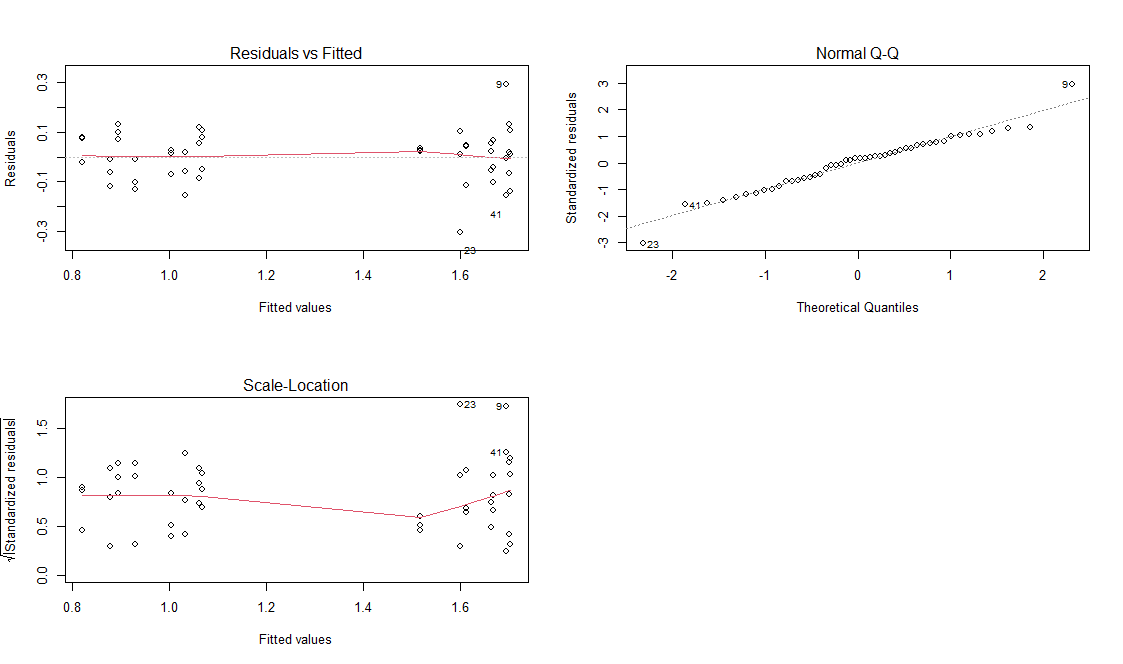
\includegraphics[width=0.8\textwidth]{images/model.png}
    \legend{Fonte: Autores.}
    \label{fig:residuos-plot3}
  \end{figure}

  No modelo gerado, foi obtido um valor de $R^2$ múltiplo de 0.9062, ou seja, o modelo pode explicar 90.62\% da variabilidade total, e o valor obtido do $R^2$ ajustado é 0.902. 

\section{Utilizando a correlação de dados}
\label{sec:verificacao_do_modelo_utilizando_a_correlacao_de_dados}

%! Escrever sobre código usado para correlacionar os dados preditos com os encontrados no segundo experimento

Em seguida, foram utilizados como dados de entrada as alturas utilizadas no segundo experimento, e em seguida submetidas ao modelo gerado no primeiro experimento. Em seguida, os resultados obtidos com esta predição foram comparadas aos dados empíricos obtidos no segundo experimento, utilizando a correlação de Pearson. 

\section{O resultado}
\label{sec:verificacao_do_modelo_o_resultado}

%! Escrever sobre o resultado encontrado e o que ele nos informa

O resultado encontrado indica que o modelo gerado no experimento foi capaz de obter uma correlação de 0.9880744 com os testes empíricos. Estes experimentos significam que o modelo gerado foi capaz de descrever o helicóptero com um modelo matemático que se assemelha bastante aos resultados reais, obtidos em teste. Os gráficos gerados da correlação, comparando as predições feitas no primeiro modelo com os resultados dos testes estão representados na Figura~\ref{fig:corr}.

\begin{figure}[H]
    \centering
    \caption{Gráficos da correlação entre o modelo gerado e testes empíricos.}
    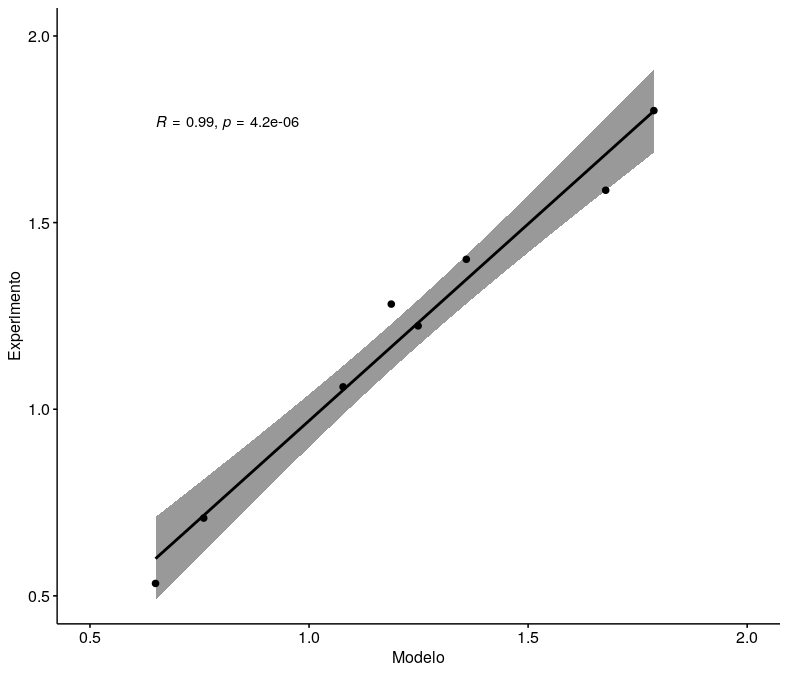
\includegraphics[width=0.8\textwidth]{images/corr.png}
    \legend{Fonte: Autores.}
    \label{fig:corr}
  \end{figure}